\chapter{系统实现}

本章基于上一章的需求分析及概要设计,介绍系统各个模块的详细设计及具体实现。我们通过
用例图、流程图、类图等方式来展示系统模块的功能及交互关系。

\section{模块化设计}

一般用户在登录后可以上传视频并进行编辑、查询与管理编辑结果,并且可以查看开发者的相关信息。用户用例图如~\ref{fig:user-uml}所示。
\begin{figure}[ht]
    \centering
    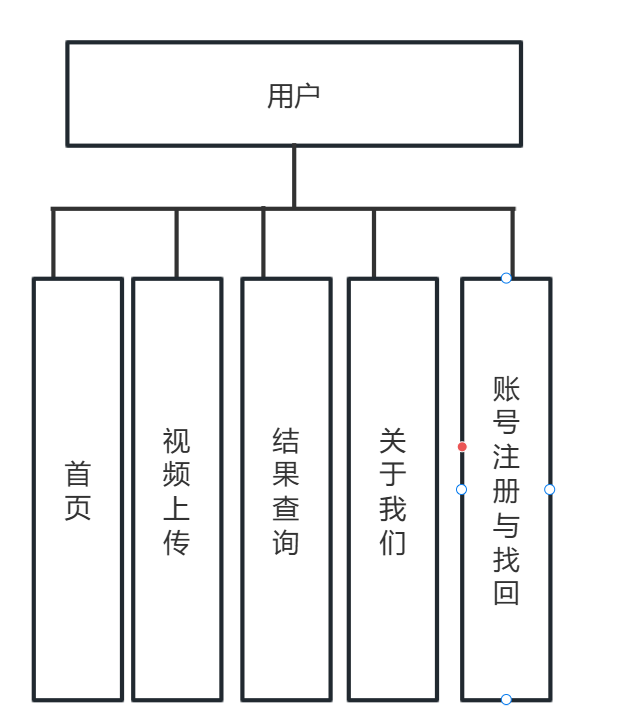
\includegraphics[width=0.3\textwidth]{source/img/user_uml.png}
    \caption{用户用例图}
    \label{fig:user-uml}
\end{figure}
管理员用户除了一般用户所拥有的功能之外,还添加了数据统计与任务请求导出功能,以方便实验室研究者了解用户真实需求。管理员用户用例图如\ref{fig:admin-uml}所示。
\begin{figure}[ht]
    \centering
    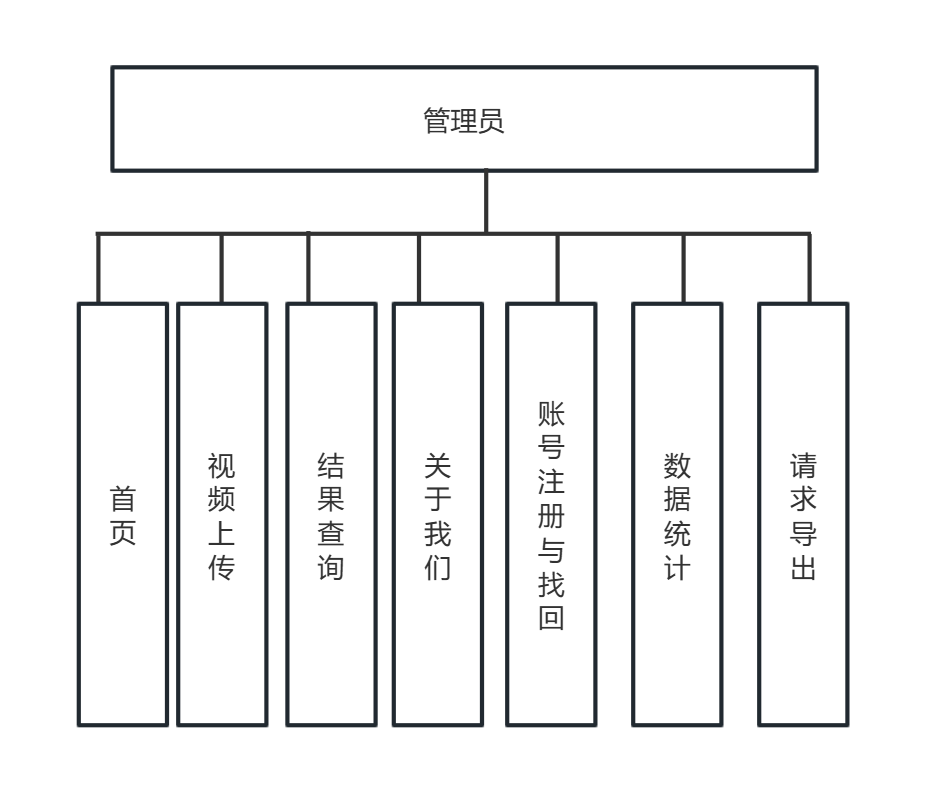
\includegraphics[width=0.4\textwidth]{source/img/admin_uml.png}
    \caption{管理员用例图}
    \label{fig:admin-uml}
\end{figure}

从用例图~\ref{fig:user-uml}和~\ref{fig:admin-uml}分析得出,系统的模块可以划分为:
\begin{itemize}
    \item 首页:作为各个功能模块的入口,完成其他各模块的合理布局;
    \item 用户管理模块:包括用户的注册、登录、注销、密码重置与找回功能;
    \item 任务上传模块:系统的核心功能,完整实现编辑任务上传的全流程;
    \item 结果管理模块:用户在该模块下查询编辑任务的结果,并提供删除、重命名等操作;
    \item 关于我们模块:展示开发者的相关信息;
    \item 数据统计模块:管理员用户在该模块下可以查看用户上传任务的数量、编辑任务的数量、编辑任务的结果数量等数据统计,并导出用户请求数据;
\end{itemize}

本节将介绍系统各个模块的具体实现,包括前端页面、后端接口、数据库设计等。由于首页只作为其余功能模块的载体,
只涉及到前端页面的布局设计,不涉及到与后端的交互;而关于我们模块作为信息展示,仅仅为静态HTML页面,我们也不再详细介绍。
另外,由于各个模块的后端操作都涉及到数据库操作,我们将数据库功能实现单独列出,不再在每个模块中介绍。

\section{首页的详细设计与实现}

在前端UI设计中,我们采用Ant Design(Antd)来辅助开发。Antd是一个基于React的UI组件库,提供高质量的React组件,并拥有完整的类型定义文件。

首页的布局采用Antd的Layout组件,使用侧边布局,在左侧放置导航栏以显示各个功能模块,如~\ref{fig:app-dashboard}所示。功能模块间的切换功能通过维护一个全局的
组件状态selectedMenu来实现,导航栏的每一项对应selectedMenu的一个值,检测到用户点击动作时,更新状态为对应的值。

\begin{figure}[ht]
    \centering
    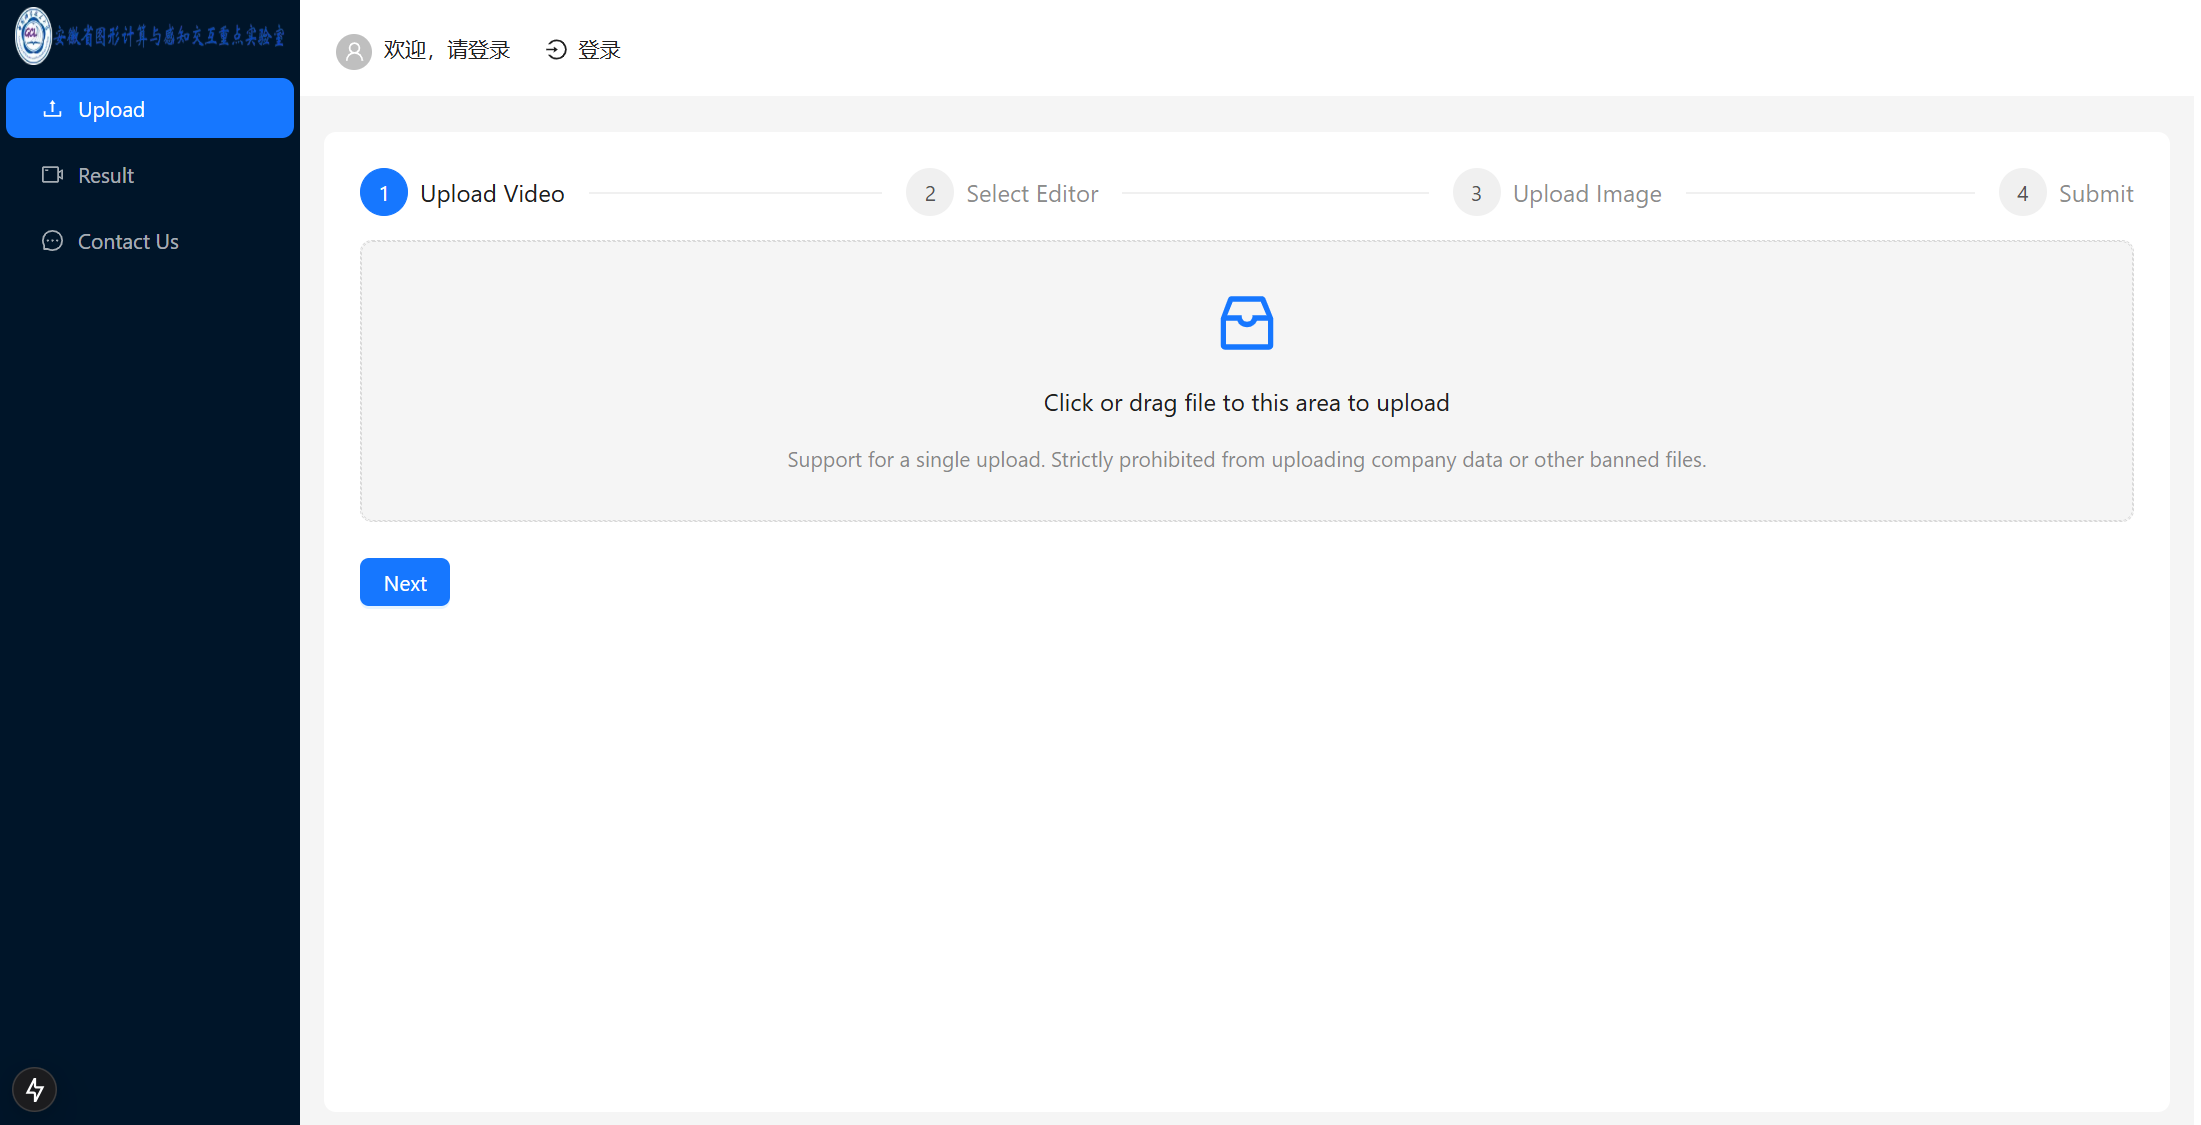
\includegraphics[width=0.8\textwidth]{source/img/app_dashboard.png}
    \caption{首页布局}
    \label{fig:app-dashboard}
\end{figure}

为了显示对应模块的内容,我们在Layout组件的Content区域设置条件渲染,根据组件状态selectedMenu的值来渲染不同的组件。
例如selectedMenu的默认值是1,对应任务上传模块,首页默认渲染任务上传组件。此外首页根据用户是否为管理员对导航栏也
进行条件渲染,只有管理员用户才能显示额外的数据统计模块。

\section{用户管理的详细设计与实现}

\subsection{流程设计}

我们设计的用户登录流程如\ref{fig:login-process}所示,图中包含我们需要实现的三个子流程:用户注册、用户登录与密码找回。
\begin{figure}[ht]
    \centering
    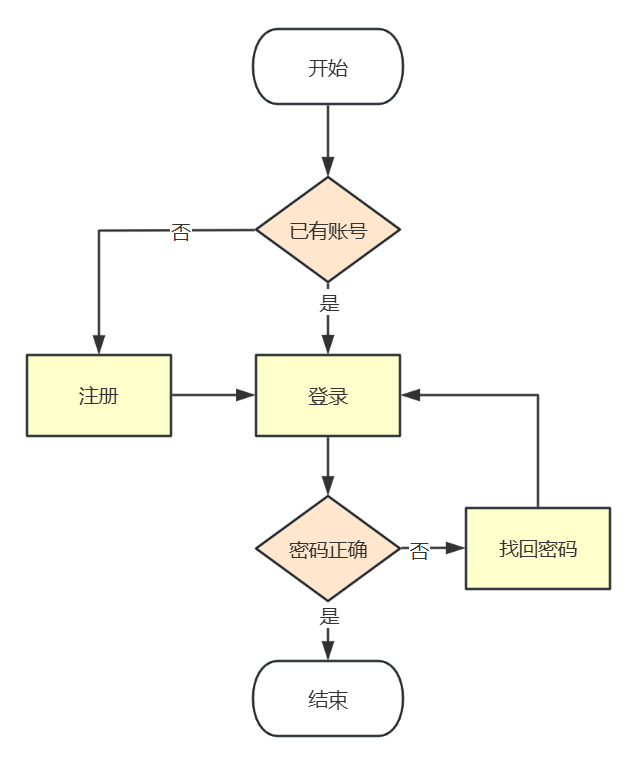
\includegraphics[width=0.4\textwidth]{source/img/login_process.png}
    \caption{登录流程图}
    \label{fig:login-process}
\end{figure}

\subsection{前端实现}

我们分别为这三个子流程设计了路由页面,并在页面中设置了路由跳转,保证用户页面跳转的双向性。我们使用Antd的Form组件来实现
表单的创建,我们通过设置组件成员的rules属性来设置表单内容检查,包括密码长度、密码复杂度、邮箱是否合法等;
组件中封装的提交按钮通过绑定自定义触发函数以处理提交事件,触发函数的主要逻辑为将后端api需要的数据封装为json格式,
通过axios发送post请求到后端,并处理返回结果。

由于系统中结果查询、上传限制查询等功能都需要使用用户信息,我们又无法频繁地要求用户录入信息,因此在登录流程中,
我们需要维护全局的用户状态以供其他模块使用。为了携带cookies信息到全局,我们选择了使用localStorage来存储用户信息,
在用户登录成功后,我们存储全局的用户信息并设置过期时间,在用户登出时,我们清除全局的用户信息。当其他模块需要使用
用户信息时,只需要从localStorage中解析出所需要的字段即可。

密码找回功能由于涉及到敏感信息,存在安全风险,因此我们设计了两步找回方式。我们需要用户输入邮箱,验证邮箱验证码通过后
自动跳转到密码重置页面,并由后端返回token,用户在重置密码时需要携带token,后端验证token后才能重置密码。这种设计可以防止
用户直接进入重置密码路由对数据库进行攻击,相比于临时生成动态路由,避免了动态路由规则被暴力破解的风险。

\subsection{后端实现}

后端主要实现的功能包括验证邮件发送、token生成与验证、密码的加密与验证。

\subsubsection{邮件发送}
邮件发送的时序逻辑图如~\ref{fig:SMTP-sequence}所示,我们在后端创建一个SMTP对象,在全局config中配置发送SMTP服务器的相关信息。
在用户注册时,我们发送一个随机生成的6位数,并同时返回前端,在前端验证用户验证码的正确性以判断是否进行下一步操作。

\begin{figure}[ht]
    \centering
    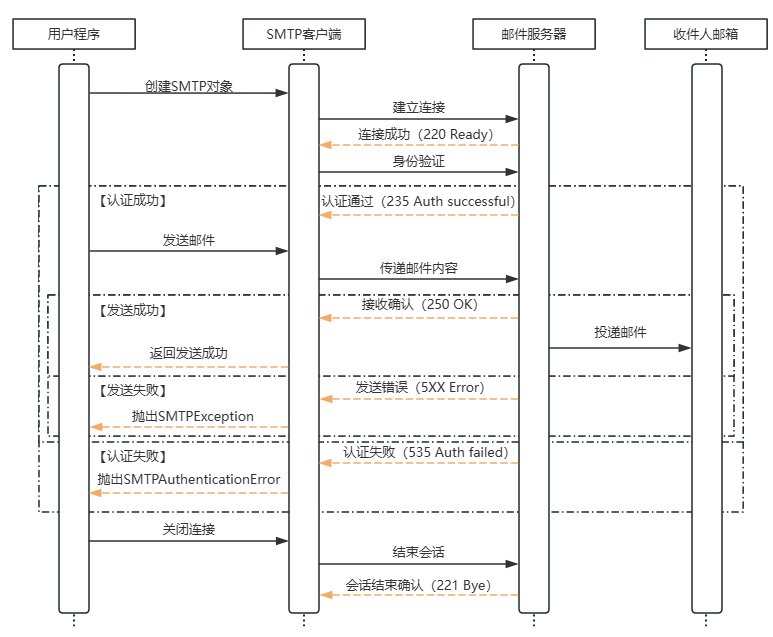
\includegraphics[width=0.6\textwidth]{source/img/SMTP_sequence.png}
    \caption{邮件发送时序图}
    \label{fig:SMTP-sequence}
\end{figure}

\subsubsection{token生成与验证}
token的生成与验证部分我们使用了JSON Web Token(JWT)库,JWT是一种用于在各方之间安全地传输信息的紧凑、URL安全的方法。
我们使用HMAC SHA256作为加密算法,在全局config中配置加密密钥,在token载荷部分存储用户信息,在找回密码时将token返回前端;
在重置密码时API要求携带token,从token中解码出用户信息后才能进行密码重置操作。

\subsubsection{密码的加密与验证}

我们将用户信息存储在数据库中,包括用户名、密码、邮箱等敏感信息。为了保证用户信息的安全性,需要对输入信息加密后存储。
我们使用密钥派生函数(Key Derivation Function, KDF)将用户提供的弱密码根据一些额外参数生成强密码,具体来说,
将用户的密码与给定的盐值(salt)连接起来,利用SHA256等加密函数经过多轮迭代得到最终的密码哈希值。由于哈希函数
具有单向性,无法通过哈希值反推原始密码,因此在验证用户密码时,我们只能重新计算哈希值并与存储的哈希值进行比较。

这种加密方式通过刻意使密钥派生的速度变慢,增加暴力破解的难度;同时由于不同密钥对应的盐值不同,确保了即使相同的密码
也会产生不同的哈希值,能够抵抗彩虹表攻击。

\section{任务上传的详细设计与实现}

\subsection{流程设计}

根据视频编辑算法的输入,需要用户提供视频、编辑提示类型与对应的提示内容,并提供邮箱以获取编辑结果。上传流程如\ref{fig:upload-process}所示。
\begin{figure}[ht]
    \centering
    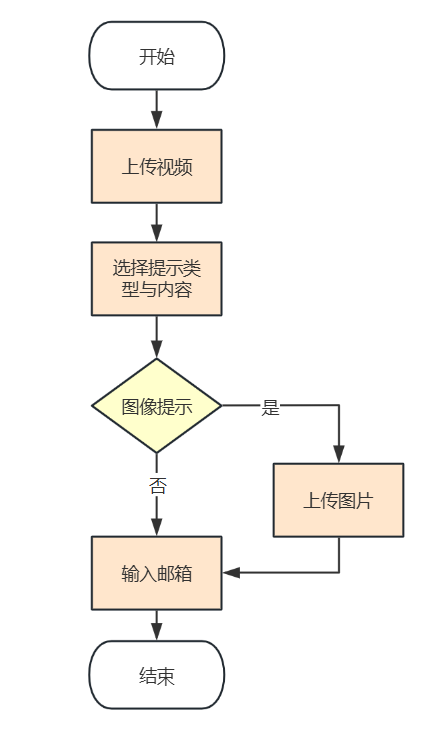
\includegraphics[width=0.3\textwidth]{source/img/edit_process.png}
    \caption{上传流程图}
    \label{fig:upload-process}
\end{figure}

\subsection{前端实现}

考虑到用户的工作流,我们使用Antd的Steps组件来展示上传流程,将上传流程分为上传视频、编辑提示、图片上传与请求提交四个步骤,
我们将这些子组件作为一个对象列表传递给Steps组件的items属性。与主页中导航栏的设计类似,我们使用组件状态current来维护当前步骤,
并将设置current状态的函数绑定在Next与Cancel两个按钮上。

注意到根据提示选择是否为Image Prompt,current状态需要决定是否跳过图片上传步骤,因此在编辑提示子组件中,
我们需要将表单中的值状态提升到父组件中,这种设计通过在子组件添加回调函数来完成。我们在子组件中加入一个提交按钮,
检测到用户点击事件后调用回调函数,从而将子组件的状态提升。

\subsection{后端实现}

后端主要实现了文件上传及管理、任务提交与分发,并调用PortraitGen算法接口。

\subsubsection{文件管理}

前端收到用户的文件提交后,通过axios发送formData格式的数据到后端API,后端将其存储到static目录下。为了方便后端对
文件的引用,并确保文件名称的唯一性,我们使用uuid库生成一个随机文件名作为文件唯一标识符。

文件管理设计的一大方面是文件过期策略,根据我们实现的上传流程,用户中途点击cancel推出后,已经上传的文件将停留在服务器上,
但用户无法再使用这些文件。因此我们在数据库中用过期时间字段来标记文件是否过期,当文件被上传时,过期时间默认设置为当前时间
的一小时后;文件被引用后,出于避免后台文件堆积的情况,我们没有永久保留这些使用过的文件,而是将过期时间延长一个月。这种设计
防止了用户短时间内大量上传文件导致后台服务器瘫痪。

为了实现过期文件删除,我们还需要运行一个后台任务。利用python的APScheduler定时任务调度框架,我们实例化了一个后台任务,
在应用初始化时同时初始化该调度器。在调度器上设置了每10秒运行文件清理,当检查到数据库中存在过期文件记录时根据路径将文件删除,
并删除数据库记录,打印删除日志。

\subsubsection{任务提交与分发}

我们使用Redis作为任务队列来管理任务。用户提交任务请求后,后端解析任务信息并通过管道操作将任务加入Redis队列,并将成功发送的结果
返回给前端。Redis在初始化时同时启动后台线程,实例化数个任务处理器,每个处理器阻塞式地获取任务,以不断地从任务队列中取出任务。
任务处理器获取任务后,调用PortraitGen算法接口,在算法对象中通过subprocess启动子进程,执行算法脚本,并将结果返回给任务处理器。

\section{结果管理的详细设计与实现}

\subsection{前端实现}

结果管理模块主要展示了用户提交的任务列表,包括任务名、任务描述、任务创建时间与完成时间、任务状态与任务结果,
并提供任务的浏览、重命名与删除功能,如~\ref{fig:app-result}所示,未完成任务的略缩图使用默认占位。
我们使用Antd的ProList组件展示任务列表,任务渲染的规则通过ProList组件属性直接全局修改。

\begin{figure}[ht]
    \centering
    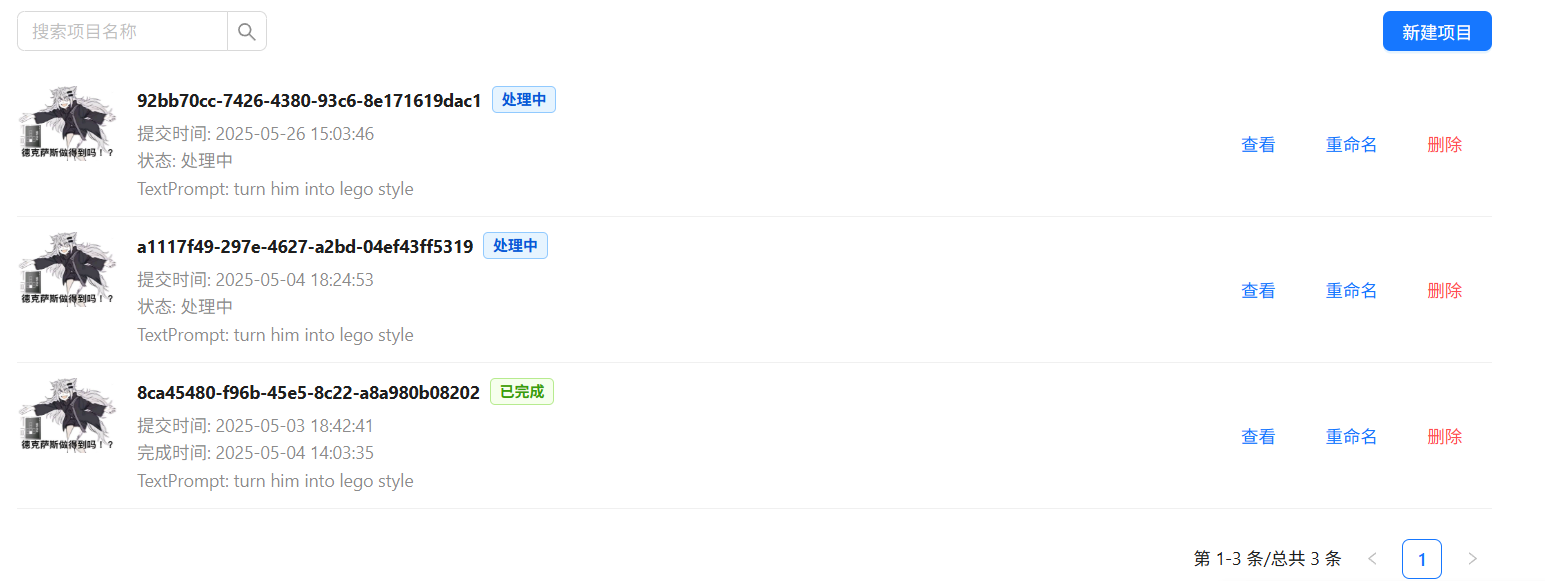
\includegraphics[width=0.8\textwidth]{source/img/app_result.png}
    \caption{结果管理页面}
    \label{fig:app-result}
\end{figure}

\subsection{后端实现}

后端操作依靠数据库的查询与更新来实现,利用MySQL数据的过滤条件,可以支持对任务的完全匹配与部分匹配查询。删除任务时,
为了防止数据库与文件系统数据不一致,我们利用事务机制,先删除数据库记录,再删除文件,如果删除文件失败则回滚事务。

\section{数据统计的详细设计与实现}

数据统计部分我们从数据库中统计用户数量、近一周上传任务及总任务数量。为了方便按照时间筛选和编辑提示类型筛选,我们设计了两种
过滤方式,另外我们提供一键导出csv功能,便于管理员进一步分析统计结果,如~\ref{fig:app-admin}所示。

\begin{figure}[ht]
    \centering
    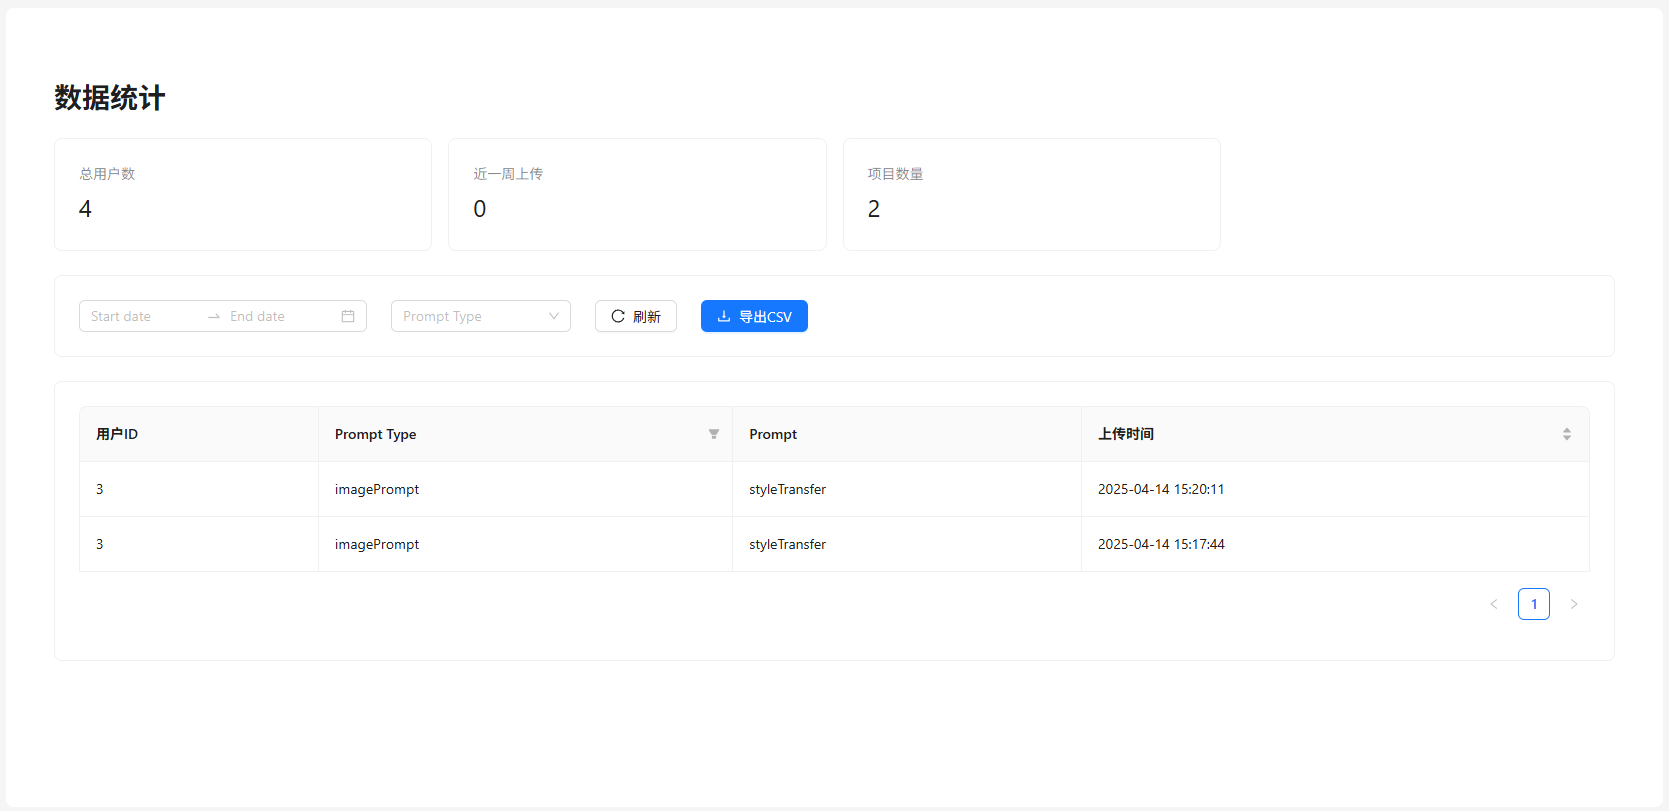
\includegraphics[width=0.8\textwidth]{source/img/app_admin.png}
    \caption{数据统计页面}
    \label{fig:app-admin}
\end{figure}

\section{数据库功能实现}

我们使用PyMySQL作为Flask框架下的MySQL数据库驱动,受到SQLAlchemy等ORM驱动框架将数据库操作封装为对象方法的启发,我们
将常用的数据库操作封装为函数,以方便在Flask应用中调用。

我们还在数据库中添加了连接池设计,以提高数据库连接的效率。由于MySQL数据库是通过TCP协议进行通信的,因此每次建立连接都需要进行三次握手,
以实现TCP的可靠传输;而建立TCP连接后数据库还需要传输认证包用于用户验证,因此数据库连接的建立是一个相对耗时的操作。我们采用的连接池设计
通过维护一定数量的数据库连接,在需要时直接从连接池中获取数据库连接,避免了频繁建立数据库连接带来的性能问题。